 \documentclass{llncs}
 \usepackage{amsmath}
\usepackage{amssymb}
\usepackage{graphicx}
\usepackage{enumerate}
\usepackage{url}

\newcommand{\tup}[1]{\langle #1 \rangle}
\newcommand{\vvec}[1]{\mathbf{#1}}
\newcommand{\join}{\bowtie}
\newcommand{\R}{\mathcal{R}}
\newcommand{\Q}{\mathcal{Q}}
\newcommand{\qrule}{:\!\!-}
\newcommand{\orule}{\sqsubseteq}
\newcommand{\mcdsat}{\textsc{McdSat}}
\newcommand{\minicon}{{MiniCon}}
\newcommand{\Omit}[1]{}

% flights
\newcommand{\flight}{\text{\it flight}}
\newcommand{\UScity}{\text{\it uscity}}
\newcommand{\national}{\text{\it national}}


\newcommand{\trip}{\textit{trip}}
\newcommand{\planetrip}{\textit{plane-trip}}
\newcommand{\traintrip}{\textit{train-trip}}
\newcommand{\AAflight}{\textit{AA-flight}}
\newcommand{\UAflight}{\textit{UA-flight}}
\newcommand{\ATtrain}{\textit{AT-train}}
\newcommand{\UPtrain}{\textit{UP-train}}
\newcommand{\train}{\textit{train}}

% Constants
\renewcommand{\AA}{\text{AA}}
\newcommand{\UA}{\text{UA}}
\newcommand{\AT}{\text{AT}}
\newcommand{\UP}{\text{UP}}
\newcommand{\PA}{\text{Paris}}
\newcommand{\NY}{\text{NY}}
\newcommand{\LA}{\text{LA}}
\newcommand{\AL}{\text{AL}}

% Services
\newcommand{\nationaltlight}{\textit{nat-flight}}
\newcommand{\onewayflight}{\textit{one-way-flight}}
\newcommand{\nationaltrain}{\textit{nat-train}}
\newcommand{\onewayTrain}{\textit{one-way-train}}
\newcommand{\onestop}{\textit{one-stop}}
\newcommand{\toPA}{\textit{to-pa}}
\newcommand{\onestopPA}{\textit{onestop-to-pa}}
\newcommand{\fromNY}{\textit{from-ny}}
\newcommand{\fromLA}{\textit{from-la}}

\begin{document}
\allowdisplaybreaks
\title{STEREO: a SaT-based tool for an optimal solution of the sERvice selEctiOn problem}
\author{Daniel Izquierdo \and Mar\'{\i}a-Esther Vidal \and Blai Bonet}
\institute{Departamento de Computaci\'on \\
           Universidad Sim\'on Bol\'{\i}var \\
           Caracas 89000, Venezuela \\
           \url{{idaniel,mvidal,bonet}@ldc.usb.ve}}
\maketitle

\begin{abstract}
We present STEREO, a system that offers an expressive formalism and implements techniques firmly grounded on logic to solve the Service Selection Problem (SSP).
STEREO adopts the Local-As-View approach to represent services' functionality as 
views on ontology concepts, while user requests are expressed as conjunctive queries on these concepts. Additionally,  users can describe their preferences, which  are  used to rank the solutions. 
We discuss the LAV formulation  of SSP; then, we illustrate the encoding of SSP  as a logical theory  whose models are in correspondence with the problem solutions, and in presence of preferences, whose best models are in correspondence with the best-ranked solutions.  We demonstrate how by exploiting properties of  modern SAT solvers, STEREO provides an efficient and scalable solution  to  SSP. 
\end{abstract}

\section{Introduction}
Nowadays, several annotation tools like the one proposed by Ambite et al.\ \cite{AmbiteISWC09}, are able to label and convert existing Web data sources into Semantic Web Services.
Once this tremendous amount of services becomes available, users
will more than ever require approaches to precisely express their selection needs and to effectively identify the services that best meet their requirements.
In order to achieve this goal, we developed  STEREO, a system that offers an expressive formalism for describing Web services and user requests,  and implements a logic-based solution to efficiently select the services that best meet the user requirements. The STEREO formalism and the techniques have been reported in  \cite{IVB2010}.
 
 STEREO is tailored to constantly changing Web service datasets and a relatively stable set of ontology concepts. STEREO adopts  the recent approach of Ambite et al.\ \cite{AmbiteISWC09}
that describes services as views on ontology concepts following the Local-As-View (LAV) approach that is widely used in integration
systems~\cite{levy:bucket}. Thus, every time that a service changes or
a new one becomes available, only a tiny fraction of the mappings
must be updated. Additionally,   STEREO models user requests  as conjunctive queries on the ontology concepts and casts  SSP  as the problem
of rewriting a query in terms of a set of views, the so-called Query
Rewriting Problem (QRP). Thus, STEREO exploits existing scalable and efficient techniques that have been proposed in the data integration area~\cite{arvelo:aaai06,levy:bucket,pottinger:minicon}.
Furthermore, STEREO offers a simple yet expressive language for preferences and supports users' preferences and constraints on the set of the
selected services to serve a given request. 
These preferences and constraints further refine and rank 
the set of valid rewritings of the posed query, in a way that
the best solution to the SSP corresponds to the best-ranked 
valid rewritings of the corresponding QRP. STEREO  constructs a propositional logical theory  that captures 
the features associated with SSPs; each model of the theory encodes a valid combination of services, and these models are ordered by their rank and the best-ranked
models are the models with minimum rank. Knowledge encoded in the ontology is used to extend the rules in the logical theory to permit the cover of ontology symbols in
the query with symbols in the views according to subsumption relationships represented in the ontology. 
We will demonstrate the benefits of the proposed approach and show the following key issues: (a) we illustrate the expressiveness of the approach; we discuss scalability  by demonstrating how STEREO is able to enumerate realistic instances of SSP in a few seconds; and finally, we demonstrate the performance  by enumerating in the same logical theory, the optimal models based on different cost/rewards of the users' preferences.  The demo is published at \url{www.ldc.usb.ve/STEREO}.
 
\section{STEREO Architecture}
\begin{figure}[t]
\centering
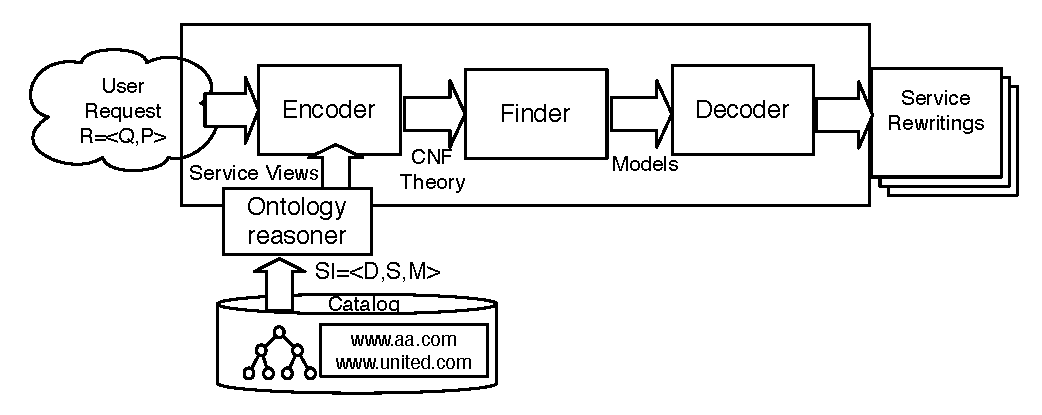
\includegraphics[height=30mm,width=.6\textwidth]{architecture.pdf}
\caption{The STEREO Architecture}
\label{fig:architecture}
\end{figure}

 The STEREO architecture  is comprised of a Catalog of service descriptions,
 an Ontology Reasoner, the Encoder, the best model Finder,
and the Decoder.
Figure~\ref{fig:architecture} depicts the overall architecture. In STEREO, an instance of SSP consists of an integration framework $IS=\tup{D,S,M}$ where $D$ is an ontology, $S$ is the set
of services, and $M$ is the set LAV mappings. A user request is a tuple $R=\tup{Q,P}$ comprised of a query $Q$  and a set of preferences $P$. The STEREO Catalog is populated with the components of the integration framework. The Ontology Reasoner computes the transitive
closure of the ontology subsumption relationships, and the Encoder module makes used of this information in conjunction with the LAV mappings,  constant symbols,   and user's preferences to encode  an input instance of SSP as a CNF theory.
STEREO uses  c2d (\url{http://reasoning.cs.ucla.edu/c2d}) to compute all the
best-ranked models of a propositional theory  in a certain 
normal form called deterministic and decomposable negation normal
form (d-DNNF) \cite{darwiche:d-dnnfs}; however, the formalization can be also used in Weighted-Max-SAT solvers.
 The Finder computes a best model by enumerating its models  and it can reuse the same d-DNNF for different cost/rewards associated with the preferences to calculate  the best service rewritings. 
   Finally, the Decoder translates the model(s)  into the input instance.


\section{Demonstration of Use Cases}
In this demonstration, we illustrate our approach on  a simple travel-information system that contains information about
flight and train trips between cities and information about which cities
are in the US. The ontology is comprised of the predicates
$\trip$, $\flight$, $\train$ and $\UScity$.
The first predicate relates cities $(x,y)$ if there is a direct
trip either by plane or train between them. The flight predicate relates $(x,y,t)$ whenever there is a direct flight from $x$ to $y$ operated by airline $t$, and similarly for $\train$,
and $\UScity$ indicates if a given city is or not a US city. 
The ontology axioms capture two subsumption relations:
\begin{alignat*}{1}
\flight(x,y,t)\  \orule\ \trip(x,y).\  & \train(x,y,t)\  \orule\ \trip(x,y).
\end{alignat*}
For the services, we assume the following type of data sources:
\begin{enumerate}[--]
\item $\nationaltlight(x,y)$ relates two US cities that are connected by a direct flight,
\item $\onestop(x,y)$ relates two cities that are connected by a one-stop flight,
\item $\nationaltrain(x,y)$ relates US cities that are connected by a direct train,
\item $\toPA(x)$ tells if there is a direct flight from $x$ to Paris,
\item $\fromLA(x)$ tells if there is a flight from Los Angeles to $x$.
\end{enumerate}

Based on the ontology concepts the services are described using LAV views:
\begin{alignat*}{1}
\nationaltlight(x,y)\ &\qrule\ \flight(x,y,t),\,\UScity(x),\,\UScity(y)\,, \\
\toPA(x)\             &\qrule\ \flight(x,\PA,\AA)\,, \\
\fromLA(x)\           &\qrule\ \flight(\LA,x,\UA)\,, \\
\onestop(x,z)\          &\qrule\ \flight(x,y,t),\,\flight(y,z,t)\,, \\
\nationaltrain(x,y)\  &\qrule\ \train(x,y,t),\,\UScity(x),\,\UScity(y)\,. 
\end{alignat*}

Consider a user that needs to select the services able to
retrieve one-stop round trips from a US city $x$ to any city $y$ in the world and the user prefers to fly rather than to travel by train. This request is represented as follows:
\[ Q(x,y)\ \qrule\ \UScity(x),\,\trip(x,u),\,\trip(u,y),\,\trip(y,v),\,\trip(v,x)\,. \]

 This preference is modeled by assigning a high reward to the symbol $\flight$. Any rewriting of the ontology predicates in terms of the services defined by these predicates, implements the request.
In addition, rewritings comprised of services defined in terms of the symbol $\flight$ will have a higher scores than those with services on the symbol $\train$.
Thus, this rewriting is  valid and  highly ranked:
\begin{alignat*}{1}
I(x,\PA)\ \qrule\ &\nationaltlight(x,u),\,\toPA(u),\, \onewayflight(\PA,v),\,\nationaltlight(v,x)\,. 
\end{alignat*}
But, the following rewritings is not a valid solution because it maps the query variable $y$ into two different constants \PA\ and \LA\ that denote different cities:
\begin{alignat*}{1}
 I'(x,y)\  &\qrule\ \nationaltlight(x,u),\,\toPA(u),\,\fromLA(v),\,\nationaltlight(v,x)\,.
\end{alignat*}

Using this travel domain, we  consider the following scenarios:
\begin{itemize}
\item We run STEREO in three different benchmarks.   We start with a benchmark of  queries with 2
to 5 sub-goals and sets of 10 to 100 services; we show that the sets of 100
airlines with 5-stop flights can be compiled in 328 secs, 
the best model can be computed in 0.29 secs, and the enumeration of all models in 0.47 secs. We add a second  service for each airline and show that STEREO behavior remains similar. Finally, we  try services with multiple sub-goals which are randomly generated and show that the compilation time  does not grow monotonically with the number of views.  The time to find the best model 
is 0.46 secs while the enumeration of all models is about 17 hours.
\item We test the system with ontologies of different sizes. Ontologies corresponding to full binary trees of depth 2 to 7  with the predicate $\trip(x,y)$ at the root node. We show that in all cases, the compilation time  is  around 13 secs.
\item To show the reusability, we assign different cost/reward to the  preferences,  
 and demonstrate that the same d-DNNF can be used to compute the best model, while the execution time remains almost the same. 
\end{itemize}

\section{Conclusions}
In this demonstration, we will present a logical-based approach that relies on the Local-As-View (LAV) formalization \cite{levy:bucket} to solve the SSP. We will show how by using simple conjunctive rules, the functionality of services  can be defined. In addition, we will demonstrate how a propositional logic-based approach can be used to represent instances of SSP, and different scenarios where the properties STEREO will be observed by  users.  We will demonstrate that the approach can be applied to
real-sized problems, while the whole approach is only possible
when the compilation of the CNF theory into d-DNNF  succeeds.
\bibliographystyle{abbrv}
\bibliography{ref}
 \end{document}
